% !TEX program = xelatex
\documentclass[10.5pt,a4paper]{article}

\usepackage[margin=1.5cm]{geometry}
\usepackage{xeCJK}
\usepackage{fontspec}
\usepackage{titlesec}
\usepackage{enumitem}
\usepackage{hyperref}
\usepackage{xcolor}
\usepackage{tabularx}
\usepackage{graphicx}
\usepackage{tikz}
\usepackage{fontawesome5}

% 字体设置
\setCJKmainfont{Noto Serif CJK SC}
\setCJKsansfont{Noto Sans CJK SC}
\setmainfont{Noto Serif CJK SC}

% 颜色
\definecolor{primary}{HTML}{2B4C7E}
\definecolor{linkcolor}{HTML}{1A5276}

% 超链接
\hypersetup{colorlinks=true, urlcolor=linkcolor}

% 节标题样式
\titleformat{\section}{\large\bfseries\color{primary}}{}{0em}{}[\titlerule]
\titlespacing*{\section}{0pt}{6pt}{4pt}

% 去掉页码
\pagestyle{empty}

% 去掉段落缩进
\setlength{\parindent}{0pt}

% 列表样式
\setlist[itemize]{leftmargin=1.5em, itemsep=0pt, parsep=0pt, topsep=1pt}

\begin{document}

% ===== 个人信息 =====
\begin{minipage}[c]{0.18\textwidth}
  \begin{tikzpicture}
    \clip (0,0) circle (1.2cm);
    \node at (0,0) {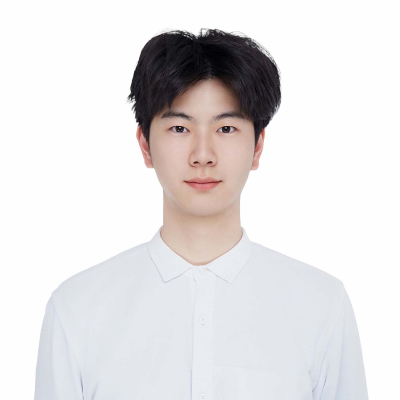
\includegraphics[width=2.4cm]{photo.jpg}};
  \end{tikzpicture}
\end{minipage}%
\hfill
\begin{minipage}[c]{0.60\textwidth}
  \begin{center}
    {\LARGE\bfseries 王思淼} \quad {\normalsize 男} \\[6pt]
    \begin{tabular}{c c c}
      \faMapMarker\ 北京 &
      \faPhone\ 13608067078 &
      \faEnvelope\ \href{mailto:mickeymiao2023@163.com}{mickeymiao2023@163.com}
    \end{tabular} \\[3pt]
    \begin{tabular}{c c}
      \faGithub\ \href{https://github.com/wangsimiao2000}{GitHub} &
      \faBlog\ \href{https://wangsimiao2000.github.io}{Blog}
    \end{tabular}
  \end{center}
\end{minipage}%
\hfill
\begin{minipage}[c]{0.18\textwidth}
\phantom{占位}
\end{minipage}

% ===== 教育背景 =====
\section{\faGraduationCap\ 教育背景}

\textbf{英国利兹大学}（QS 世界第75，2023），利兹，英国 \hfill 2023.09 -- 2024.11 \\
硕士 · 高性能图形与游戏工程（计算机科学与技术）

\vspace{3pt}

\textbf{西南石油大学}（双一流），成都，四川 \hfill 2019.09 -- 2023.06 \\
本科 · 软件工程

% ===== 工作经历 =====
\section{\faBriefcase\ 工作经历}

\textbf{北京小米移动软件有限公司} · 图形渲染开发工程师 \hfill 2025.02 -- 至今 \\
北京总部
\begin{itemize}
  \item 参与嵌入式动效引擎核心模块的设计与开发
  \item 基于动效引擎进行穿戴系统动效应用开发
  \item 参与自动化测试框架搭建，提升图形渲染模块的测试覆盖率与效率
  \item 参与 Mesh 绘制相关功能开发，优化渲染管线性能
  \item 参与 LVGL 部分接口优化
\end{itemize}

% ===== 项目经历 =====
\section{\faCode\ 项目经历}

\textbf{SnowLeopardEngine — 团队游戏引擎} \hfill 2023.09 -- 2024.06 \\
C++ · OpenGL 4.6 · PhysX · XMake \hfill \faGithub\ \href{https://github.com/SnowLeopardEngine/SnowLeopardEngine}{GitHub}
\begin{itemize}
  \item 利兹大学7人团队课程项目，开发跨平台游戏引擎，支持 PBR 渲染、骨骼动画、后处理等
  \item 负责物理模块开发，基于 NVIDIA PhysX 实现各类 Collider 碰撞检测与刚体物理模拟
  \item 使用事件回调机制实现场景中 Actor 的动态加载与销毁，参与 ImGui 编辑器 UI 开发
\end{itemize}

\vspace{3pt}

\textbf{MinecraftSkin Raytracer — MC皮肤光追渲染器} \hfill 2024 \\
C++17 · Qt6 · OpenGL \hfill \faGithub\ \href{https://github.com/WangSimiao2000/MinecraftSkin_Raytracer}{GitHub}
\begin{itemize}
  \item 独立开发纯 CPU 软件光线追踪桌面应用，将 Minecraft 皮肤渲染为高质量图像
  \item 实现 Blinn-Phong 光照、多次反射、阴影，支持基于图块的多线程并行渲染
  \item 集成 OpenGL 实时预览（轨道/自由漫游模式），支持从 Mojang API 自动获取皮肤
\end{itemize}

\vspace{3pt}

\textbf{InfiniteVoxelCaveWorld — 无限体素洞穴地形} \hfill 2024 \\
C++ · OpenGL \hfill \faGithub\ \href{https://github.com/WangSimiao2000/InfiniteVoxelCaveWorld}{GitHub}
\begin{itemize}
  \item 实现基于区块的程序化无限体素洞穴地形生成，使用 OpenSimplex2 噪声控制地形与洞穴阈值
  \item 采用体素相邻面剔除与视锥体剔除优化渲染性能，使用 GLSL 实现 Blinn-Phong 着色
  \item 多线程分离渲染循环与区块生成逻辑，集成 ImGui 实时调试界面
\end{itemize}

\vspace{3pt}

\textbf{OutlineShaderForUE — UE描边后处理Shader} \hfill 2024 \\
Unreal Engine · HLSL \hfill \faGithub\ \href{https://github.com/WangSimiao2000/OutlineShaderForUE}{GitHub}
\begin{itemize}
  \item 实现基于深度和法线的后处理描边效果，支持距离衰减、自定义深度遮罩、粗细可调
\end{itemize}

\vspace{3pt}

\textbf{利兹大学计算机图形学课程项目} \hfill 2023 -- 2024 \\
C++ · OpenGL · GLSL
\begin{itemize}
  \item 建模与渲染：蒙特卡洛路径追踪、斯涅尔定律折射、菲涅尔方程反射；法线贴图、高度图地形光栅化、Blinn-Phong 光照 \href{https://github.com/WangSimiao2000/Foundations_of_Modelling_and_Rendering}{\faGithub}
  \item 动画与模拟：骨骼动画多坐标系变换、多动画周期混合（转向/跑步/静止）、粒子系统 \href{https://github.com/WangSimiao2000/Animation_and_Simulation}{\faGithub}
  \item 几何处理：有向边数据结构、流形检测与属数计算、Loop 曲面细分、纹理映射展开 \href{https://github.com/WangSimiao2000/Geometric-Processing}{\faGithub}
\end{itemize}

% ===== 技术技能 =====
\section{\faTools\ 技术技能}

\begin{tabularx}{\textwidth}{@{} l X}
  \textbf{编程语言} & C++/C、Python \\
  \textbf{图形相关} & OpenGL、LVGL \\
  \textbf{开发工具} & Git、CMake、Linux \\
\end{tabularx}

% ===== 语言能力 =====
\section{\faLanguage\ 语言能力}

英语 · 雅思 6.0 · 朗思笔试 B2 High Pass / 口试 C1 Pass

\end{document}
